The architecture presented in this chapter was created following the Belief, Desires and Intentions (BDI) approach, as could be seen in the Figure~\ref{fig:GeneralArchitecture}  !!WRITE WHY IT WAS CHOSEN THIS APPROACH. Additionally to the modules BDI, it was added the modules of action modulation and description. The description module is used to create information that it could be used by the robot as: the script, normal speed, etc.
\begin{figure}
	\centering
	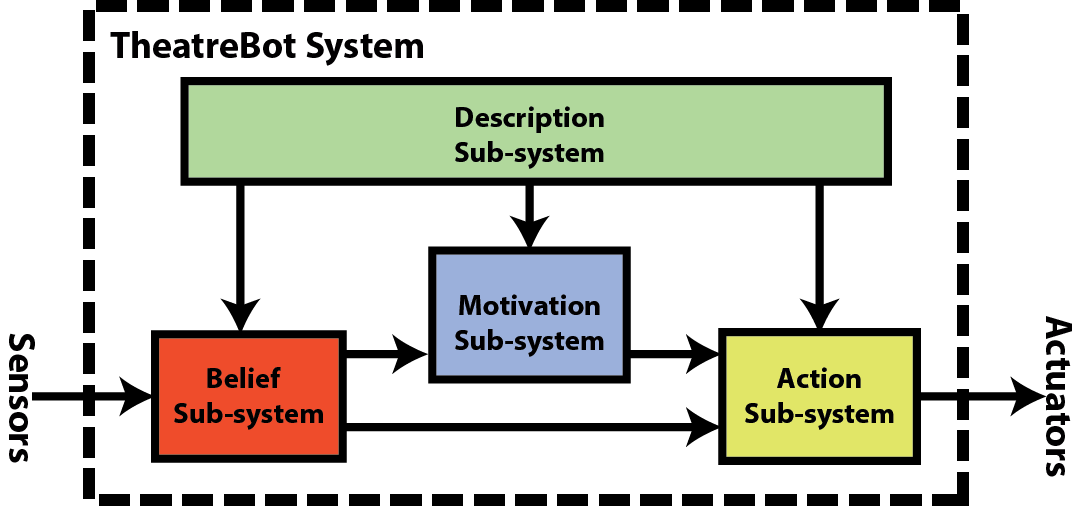
\includegraphics[width=1.0\textwidth]{./Images/Architecture/GeneralArchitecture.png} 
	\caption{General Architecture. The dash line shows the components that are in the system. The concepts of Desires and Intentions are included in the box Motivation.}
	\label{fig:GeneralArchitecture}
\end{figure}
Each of the modules are decomposed in sub-system that working as a whole could be used to accomplish the task. The final result could be seen in the Figure~\ref{fig:ArchitectureWithSubSystems}, where the module Action was divided in two: Action decision and Action modulation. Also was added the sub-module feature. Each of the modules in the architecture will be described in more detail though this chapter. 
\begin{figure}
	\centering
	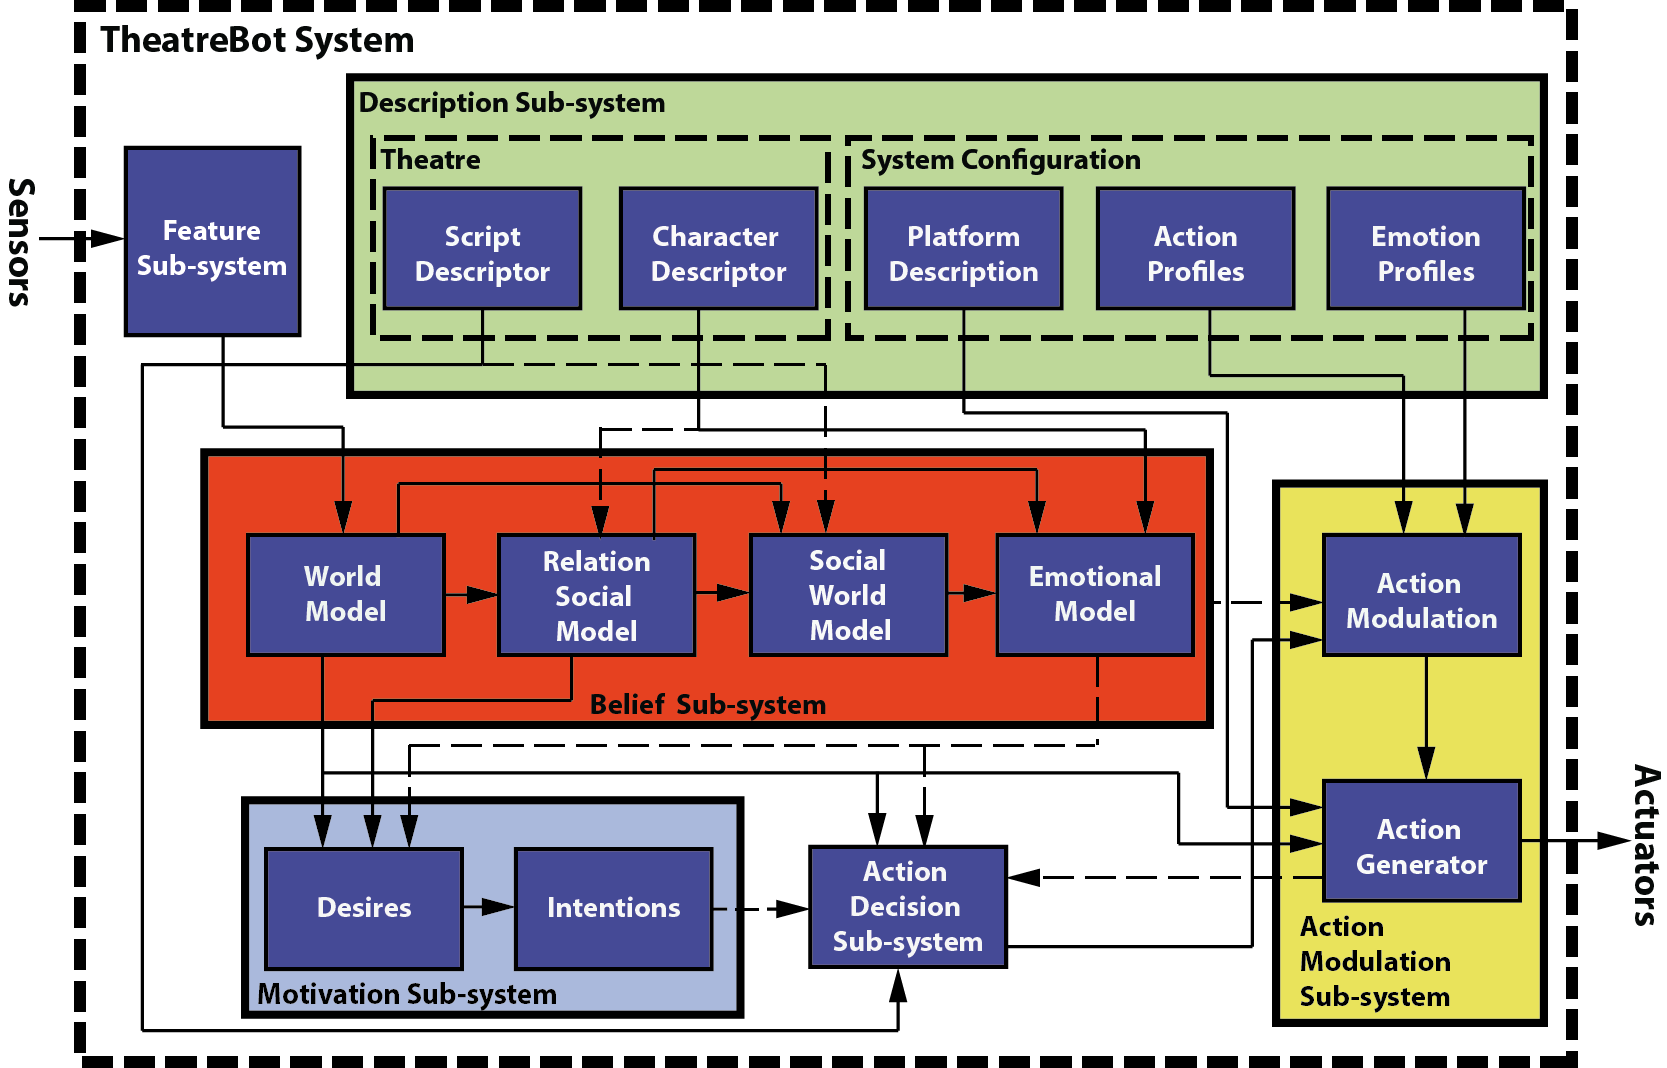
\includegraphics[width=1.0\textwidth]{./Images/Architecture/ArchitectureNew.png} 
	\caption{Architecture with the subsystems.}
	\label{fig:ArchitectureWithSubSystems}
\end{figure}
The whole action system is based on two main concepts: simple actions and abstract actions.
%%%%%%%%%%%%%%%%%%%%%%%%%
\subsection{Simple Action}
The simple actions are actions that have specialized modules that execute them. In order words they are already implemented and are platform dependent, thus it should be a different implementation of the action for the each platform that should be supported. In the first implementation, simple action should be follow the next characteristics:
\begin{itemize}
	\item Simple action controllers are not aware about other simple action controller. The synchronization is done through other module.
	\item Actions that are using the same actuators should be additive. For example the action move and oscillatemove are additive because oscillatemove is just going to introduce oscillation given an angle $theta$, thus the $theta$ could be modified by move. These actions two actions are controlled by the same controller, but its interface is different.
\end{itemize} 
At the moment the current actions are:
\begin{itemize}
	\item $Move(finalposition,trajectoryDescription)$ where finalPosition is the vector $<x,y,\theta>$ and velocity is a vector $<velocity\_x,velocity\_y,velocity\_\theta>$. The controller for this action should move the robot from its current position to the desire position. It is important to notice that the controller must also have as an input the world model in order to avoid obstacles. The trajectoryDescription is optional, thus if there is not given any information on this, the default values are used.
	\item $OscillateMove(velocity\theta,maximumAngle,trajectoryDescription)$ the oscillation movement just implies movement in the angular velocity, thus it is just change in the $\theta$ component, and $maximumAngel\in[\pi,-\pi)$
	\item $RotateTorso(angle,trajectoryDescription)$ moves the upper part of the waist, if there is one.
	\item $OscillateTorso(velocity,maximumAngle)$ which enable the oscillation of the upper part of the waist.
	\item $Grasp(object)$ try to grasp the desire object
	\item $RotateHead(angle\theta,angle\beta,angle\omega,velocity\theta,velocity\beta,velocity\omega)$
	\item $OscillateHead(angelID,velocity,angle)$ where\\ $angleID\in \lbrace angle\theta,angle\beta,angle\omega \rbrace$
	\item $RorateShoulder(IDShoulder,angle\theta,angle\beta,velocity\theta,velocity\beta)$
	\item $OscillateShoulder(IDShoulder,angleID,velocity,maximumAngle)$ where\\ $IDShoulder\in (\forall x| x=shoulder\bigwedge x\in robot)$
	\item $Speak(text)$ where $text$ is the argument that should be said by the robot
\end{itemize} 
%%%%%%%%%%%%%%%%%%%%%%%%%
\subsection{Abstract Actions}
Abstract actions are actions that could be composed by other abstract or simple actions. For the composition of these kind of actions could be used any kind of synchronization constrains and structure. For example, one abstract action could be composed by other two actions that are executed concurrently or in serially. Right now, the time constrains are not considered.\\
The abstract action $walk_speak$ which has three parameters: $position$, $trajectory_description$ and $phrase$. This actions is composed by two actions: the abstract action $walk$ and the simple action $speak$. Note that the abstract action $walk$ is also composed by two simple actions: $move_body$ and $move_shoulders$.\\
The parameters of the abstract actions are explicit attached to the parameters of the actions that composed it. However, in not all the cases the parameters are covered by the abstract actions, thus it should be given an explicit value during the implementation and give a modification through the description system.



